\appendixsection{项目材料与报告索引}\label{sec:appendix-materials}

\appendixsubsection{项目结构说明}
QuickBoard 系统由前端、后端与 OCR 服务三部分组成：
\begin{itemize}
  \item \textbf{前端 Web 应用}：基于 Vue3 + Vite 与 Fabric.js，负责用户交互与画布渲染，包含白板编辑、房间入口与公式交互等模块。
  \item \textbf{后端协作服务}：基于 Node.js（Express）与 Socket.IO，负责房间管理、实时事件分发、同步裁决与版本对齐，并提供 OCR 请求的统一代理接口。
  \item \textbf{OCR 服务}：基于 FastAPI，负责图像预处理与数学公式识别推理，并输出可插入的 LaTeX 表达。
\end{itemize}

\appendixsubsection{验证材料说明}
为保证本文结论具有可复核性，关键改动均配套记录单元测试与构建验证结果；针对同步一致性、渲染性能与过程预览降载等关键结论，均记录实验参数、原始统计与结果摘要。相关验证材料随论文一并提交，便于复核与对照。

\appendixsubsection{开题报告图片复用}
\begin{figure}[htbp]
  \centering
  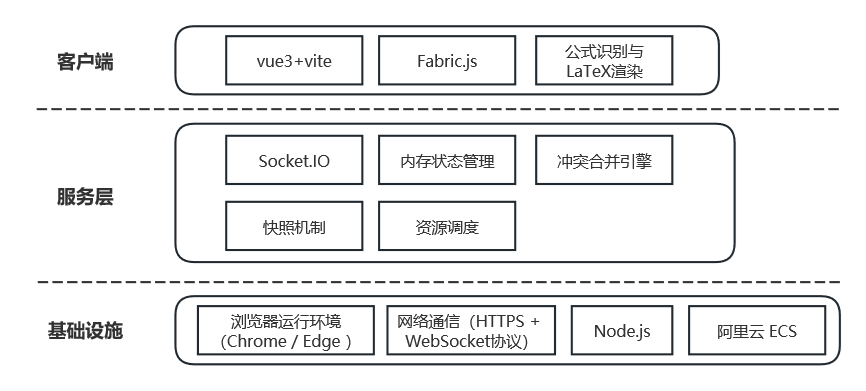
\includegraphics[width=0.92\linewidth]{figures/proposal_arch.png}
  \caption{开题报告阶段技术架构图（复用）}\label{fig:proposal-arch}
\end{figure}

\appendixsubsection{开题调研与需求分析补充}
本课题在开题阶段对短会话协作与教学场景的工具需求进行了归纳，并将需求收敛为“进入路径短、表达成本低、协作反馈及时、弱网可恢复、内容可沉淀”五类核心目标。其关键观点可概括如下。

\textbf{（1）进入路径短。} 短会话协作常发生在临时讨论与课堂推导中，参与者随时加入或离开。若系统依赖注册、团队空间配置或复杂权限设置，会显著增加进入成本并打断讨论节奏。因此系统入口优先提供创建/加入房间与复制分享链接，房间号采用纯数字便于口述与输入，最近房间用于降低重复进入成本。

\textbf{（2）表达成本低。} 白板价值在于支持图形、文本与公式等多模态表达。基础绘图工具（画笔、形状、文本、橡皮、撤销重做）覆盖了多数课堂与讨论需求；在数学场景下，公式输入需要兼顾低门槛与可编辑性，因此采用“框选识别 + 确认插入 + 二次编辑”的交互闭环，并通过错误码与 traceId 将失败原因工程化。

\textbf{（3）协作反馈及时。} 协作工具的核心体验是“我做的修改对方能立刻看到”。因此系统采用基于事件的实时通信，并将协作域抽象为房间。对象变更采用最小增量传播以降低延迟与带宽开销，并通过服务端权威裁决保证多端接收一致的裁决结果。

\textbf{（4）弱网可恢复。} 教学与远程场景中，网络抖动、丢包与断线重连不可避免。若仅依赖朴素广播，容易出现乱序覆盖与状态分叉。系统以字段级 LWW 为合并核心，并结合版本补包与快照兜底实现最终收敛；当断线窗口过大或日志不足时，退化为权威快照以保证正确性优先。

\textbf{（5）内容可沉淀。} 短会话协作虽然强调即时性，但课堂推导与讨论结果往往需要沉淀为可复用材料。系统提供导出能力与公式对象的可编辑表示，使内容能够以更稳定的形式保存与复用。

上述补充内容与正文中的需求分析相互印证，用于说明本课题在功能取舍与工程设计上的依据。
